\kommentar{Magnetostatik} %Thema

\begin{lk}{Wie gross ist die Magnetische Permeabilität des Vakums?}
	\LARGE{$ \mu_0 = 4 \cdot \pi \cdot 10^{-7} \dfrac{Vs}{Am} $ \\[12pt] $ = 1.2566  \cdot 10^{-6} \dfrac{H}{m}$}
\end{lk}

\begin{lk}{Was bezeichnet man als Induktivität?}
	Verhältnis zwischen zwei Grössen (Strom und Magnetischer Fluss), Proportionalitätsfaktor\\[12pt]
	\center{\huge{$ L = \dfrac{\phi}{I} $}}
\end{lk}

\begin{lk}{Welche Arten/Ausprägungen der Induktivität gibt es?}
	\begin{compactitem}
		\item Selbst Induktivität (Magnetischer Fluss welcher durch die Kontur der Fläche geht welche von einem stromdurchflossenen Leiter begrenzt wird)\\
		$ L = \dfrac{\phi_1}{I_1} $
		\item Gegen Induktivität (Ein Magnetischerfluss beeinflusst eine andere Kontur)\\
		$ L = \dfrac{\phi_2}{I_1} $
	\end{compactitem}
\end{lk}

\begin{lk}{Was ist der Unterschied zwischen innerer und äusserer Induktivität?}
	Innere Induktivität ist die Induktivität innerhalb des Leiters, äussere Induktivität ist die Induktivität ausserhalb des Leiters.
\end{lk}

\begin{lk}{Was wird als verketteter Fluss bezeichnet?}
	Wenn ein Magnetischer Fluss eine Fläche mehrfach durchdringt bezeichnet man dies als verketteter Fluss. ($ N \cdot \phi $)
\end{lk}

\begin{karte}{Was ist die Ampersche Kraft zwischen elektrischen Ströme?}
	\begin{itemize}
		\item Das Modell ist ähnlich zu Elektrostatik
		\item $d \vec{F}=\dfrac{\mu_{0}}{4 \pi} \dfrac{\left(I_{1} d \vec{l_{1}}\right) \cdot\left(I_{2} d \vec{l_{2}}\right)}{R^{2}}(-\hat{R})$
		\item Nur halbe Wahrheit. Stimmt für sehr nahe Leiter nicht mehr denn wenn $R \rightarrow 0$ dann $ F \rightarrow \infty$ und dies ist nicht korrekt.
		\item Die Richtung der Kraft lässt sich anhand der Recht-Hand-Regel ermitteln (RHR).
	\end{itemize}
\end{karte}

\begin{karte}{Wie lautet die Rechthandregel (RHR) um die Richtung der Kraft zu bestimmen?}
	\center 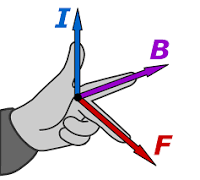
\includegraphics[width=0.5\textwidth]{pics/MS_RHR.png} %https://www.seekclipart.com/clipart/iRJbTmT_drei-finger-regel-physik-drei-finger-regel-clipart/

\begin{karte}{Was ist das Bivot Savart Gesetz und wann hat es seine Gültigkeit?}
	Mit Hilfe dieses Gesetzes kann die magnetische Flussdichte für jegliche Ströme und Stromdichten von \textbf{geschlossenen} Stromkreisen berechnet werden.
	\begin{center}
		\begin{huge}
			$d \vec{B}=\frac{\mu_{0}}{4 \pi} \frac{(\vec{J} d v) \times \hat{R}}{R^{2}}$
		\end{huge}
	\end{center}
	Dabei ist $\vec{J} d v$ der Volumenstrom.\\[5pt]
	Das Biot-Savart Gesetz gilt nur für Magnetfelder von Strömen und Stromdichten Geschlossener Stromkreise (sie können auch über die Unendlichkeit geschlossen sein)\\[5pt]
	Die Richtung kann mit der Rechtfaustregel (RFR) bestimmt werden.
\end{karte}

\begin{karte}{Was ist die Lorenzkraft?}
	Die Lorenzkraft ist die Überlagerung der elektrischen und magnetischen Kräfte\\
	\begin{center}
		\begin{huge}
			$\vec{F}=\vec{F_{E}}+\vec{F_{B}}=q(\vec{E}+\vec{v} \times \vec{B})$
		\end{huge}
	\end{center}
\end{karte}

\begin{karte}{Was bedeutet Magnetostatik?}
	\begin{itemize}
		\item Konstanten Strom (gleichmässig bewegte Ladung)
		\item Keine Zeitliche veränderliche Felder
	\end{itemize}
\end{karte}

\begin{karte}{Was bezeichnet man als Magnetfeld und was sind dessen Eigenschaften?}
	\begin{itemize}
		\item Ein Raum in welchem geladene Teilchen Kraft erfahren wenn sie sich bewegen
		\item Mathematisches und physikalisches Hilfsmittel, um ein Modell zu erstellen, um Kräfte zu beschreiben und um sie zu berechnen.
		\item Die Existenz des Magnetfelds ist nicht bewiesen, man kann nur die Auswirkungen nachweisen
		\item Das Magnetostatische Feld kann keine Arbeti verrichten, Kraft ist senkrecht zu den Feldlinien.
	\end{itemize}
\end{karte}

\begin{karte}{Was sind Pseudo Vektoren?}
	\begin{itemize}
		\item Bei Spiegelung ändert das Vorzeichen der Pseudovektoren nicht
		\item Sind keine Vektoren im Physikalischem Sinn.
	\end{itemize}
\end{karte}

\begin{karte}{Was sind die Eigenschaften vom Magnetischen Fluss?}
	\begin{itemize}
		\item Der Fluss ist kontinuierlich
		\item Keine Quellen und Senken
		\item Gaussches Gesetz des Magnetfelds
		\item Fluss ist die Summe aller Magnetischen Flussdichten welche durch eine Fläche fliessen.
	\end{itemize}
\end{karte}

\begin{karte}{Was ist das Magnetische Vektorpotential?}
	\begin{center}
		\begin{huge}
			$\vec{A}=\dfrac{\mu_{0}}{4 \pi} \dfrac{q vec{v}}{R}=\dfrac{\mu_{0}}{4 \pi} \dfrac{I \vec{l}}{R}$
		\end{huge}
	\end{center}
	Das Prinzip des elektrischen Potentials einer statischen Punktladung wird für das Vektorpotential auf dynamische Punktladungen erweitert. Wenn sich diese Ladung $q$ mit konstanter Geschwindigkeit $\vec{v}$ bewegt, kann daraus das magnetische Potential dieser bewegten Ladung definiert werden, wobei beachtet werden muss, dass es sich dabei um eine vektorielle Grösse handelt.
\end{karte}

\begin{karte}{Was bezeichnet man als Induktivität und welche Arten/Ausprägungen gibt es davon?}
	Verhältnis zwischen zwei Grössen $\left(\dfrac{Strom}{magnetischer Fluss}\right)$, Proportionalitätsfaktor\\[5pt]
	\begin{center}
		\begin{large}
			$L = \dfrac{\psi}{I}$\\[5pt]
		\end{large}
	\end{center}
	\begin{itemize}
		\item \textbf{Selbstinduktivität}: Magnetischer Fluss welcher durch die Kontur der Fläche geht durch welche auch der Strom fliesst. $L=\frac{\psi_1}{I_1}$
		\item \textbf{Gegeninduktivität}: Magnetfeld beeinflusst andere Konturen $L=\frac{\psi_2}{I_1}$
	\end{itemize}
\end{karte}

\begin{karte}{Was ist der Unterschied zwischen innerer und äusserer Induktivität?}
	Die innere Induktivität ist innerhalb des Leiters. Die äussere Induktivität ist ausserhalb des Leiters. Diesser unterschied ist vorallem wichtig bei der Selbstinduktivität.
\end{karte}

\begin{karte}{Was wird als verketteter Fluss bezeichnet?}
	Wenn ein gewisser Magnetischer Fluss eine Fläche mehrfach durchdringt.\\
	\center	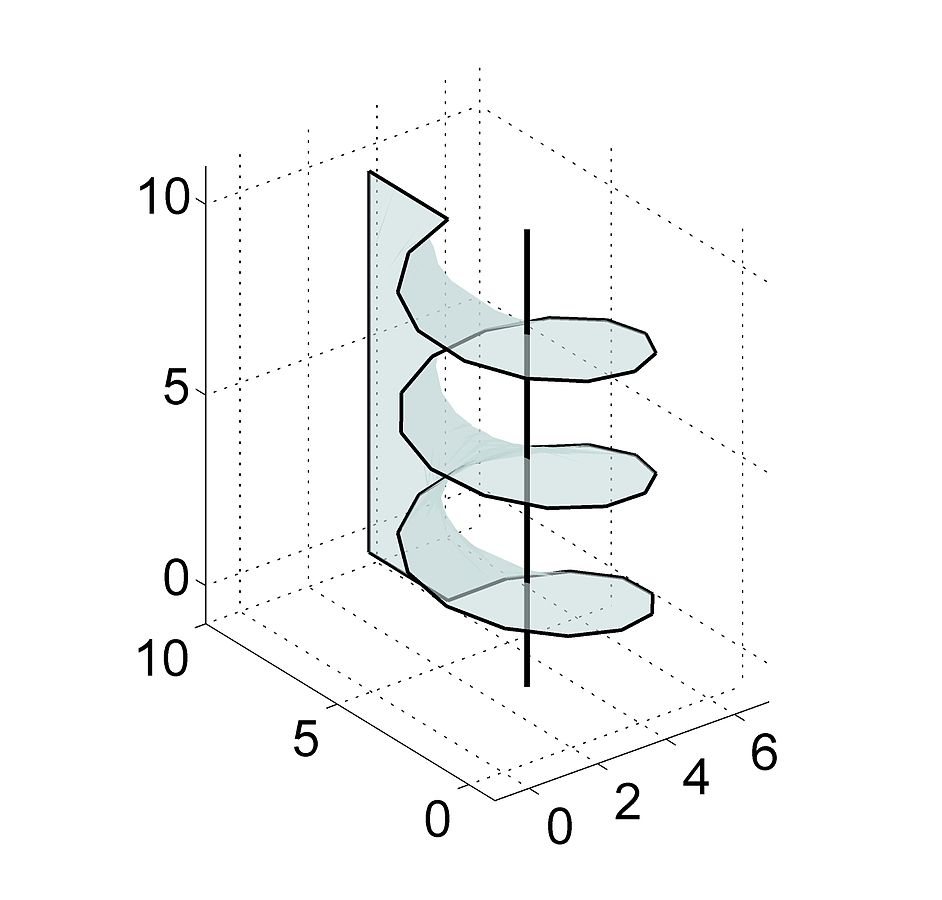
\includegraphics[width=0.4\textwidth]{pics/MS_Verketteter_Fluss.jpg} %Von Michael Lenz - Eigenes Werk, CC BY-SA 3.0, https://commons.wikimedia.org/w/index.php?curid=18760261
\end{karte}

\begin{karte}{Was bedeutet der Begriff "magnetisches Dipolmoment"?}
	Das magnetische Dipolmoment ist ein potenzielles Drehmoment wenn es ein Magnetfeld gibt.\\
	Ein Strom $I$ in einer Schleife der Fläche $A$ produziert bezüglich deren Normalenvektor $\hat{n} \perp A$ ein sogenanntes magnetisches Dipolmoment.\\
	\begin{center}
		\begin{huge}
			$\vec{m} = \hat{n} I A$
		\end{huge}
	\end{center}
	Die Flussrichtung des Stromes $I$ und die Flächennormale $\hat{n}$ sind dabei gemäss einem Rechtshandsystem miteinander verbunden.
\end{karte}

\begin{karte}{Was bezeichnet man als Magnetisierung?}
	\begin{itemize}
		\item Ausrichtung der Dipole
		\item Dipoldichte (Wo sind sie wie stark ausgerichtet)
		\item $\vec{B_M} = \mu_{0} \vec{M}$ oder $\vec{B_H} = \mu_{0} \vec{H}$ je nach Ursache
	\end{itemize}
\end{karte}

\begin{karte}{Wie ist die Magnetische Feldstärke definiert?}
	\begin{center}
		\begin{huge}
			$\vec{B} = \vec{B_M}+ \vec{B_H}= \mu_0 \left(\vec{M} + \vec{H}\right)$\\
			$\rightarrow \vec{H} = \dfrac{\vec{B}}{\mu_0} - \vec{M}$\\
		\end{huge}
	\end{center}
	Magnetischer Fluss minus Magnetisierung
\end{karte}

\begin{karte}{Welche Grenzbedinungen gelten für Magnetfelder?}
	\flushleft 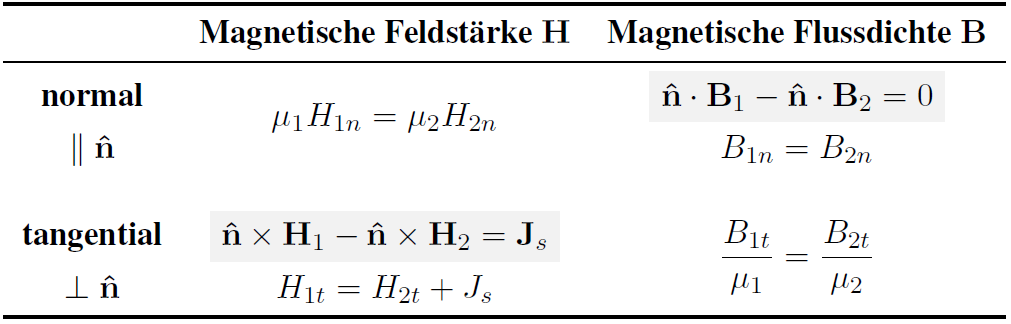
\includegraphics[width=\textwidth]{pics/MS_Grenzbedinung.png} %Quelle Skript von Hans-Dieter Lang
\end{karte}

\begin{karte}{Wie Funktioniert der Diamagnetismus?}
	\begin{itemize}
		\item Magnetisierung entgegen des äusseren Feldes
		\item Schwächt das äussere Magnetfeld (leicht)
	\end{itemize}
	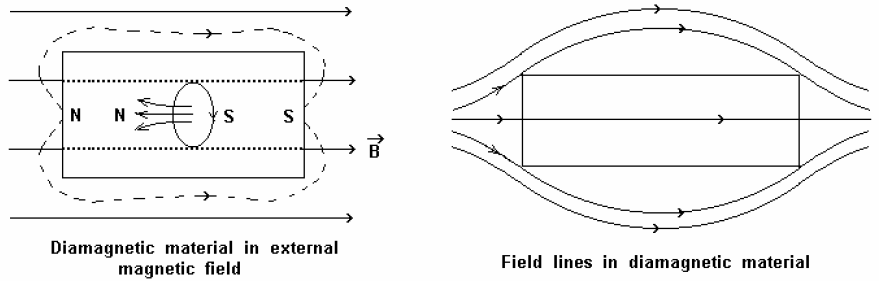
\includegraphics[width=0.9\textwidth]{pics/MS_Diamagnetismus.png} %By Nitianabhigyan - Own work, CC BY-SA 4.0, https://commons.wikimedia.org/w/index.php?curid=58224473
\end{karte}

\begin{karte}{Wie Funktioniert der Paramagnetismus?}
	\begin{itemize}
		\item Magnetisierung entlang des äusseren Feldes
		\item Stärkt das äussere Magnetfeld (leicht)
	\end{itemize}
	\begin{center}
		\begin{minipage}{0.32\textwidth}
			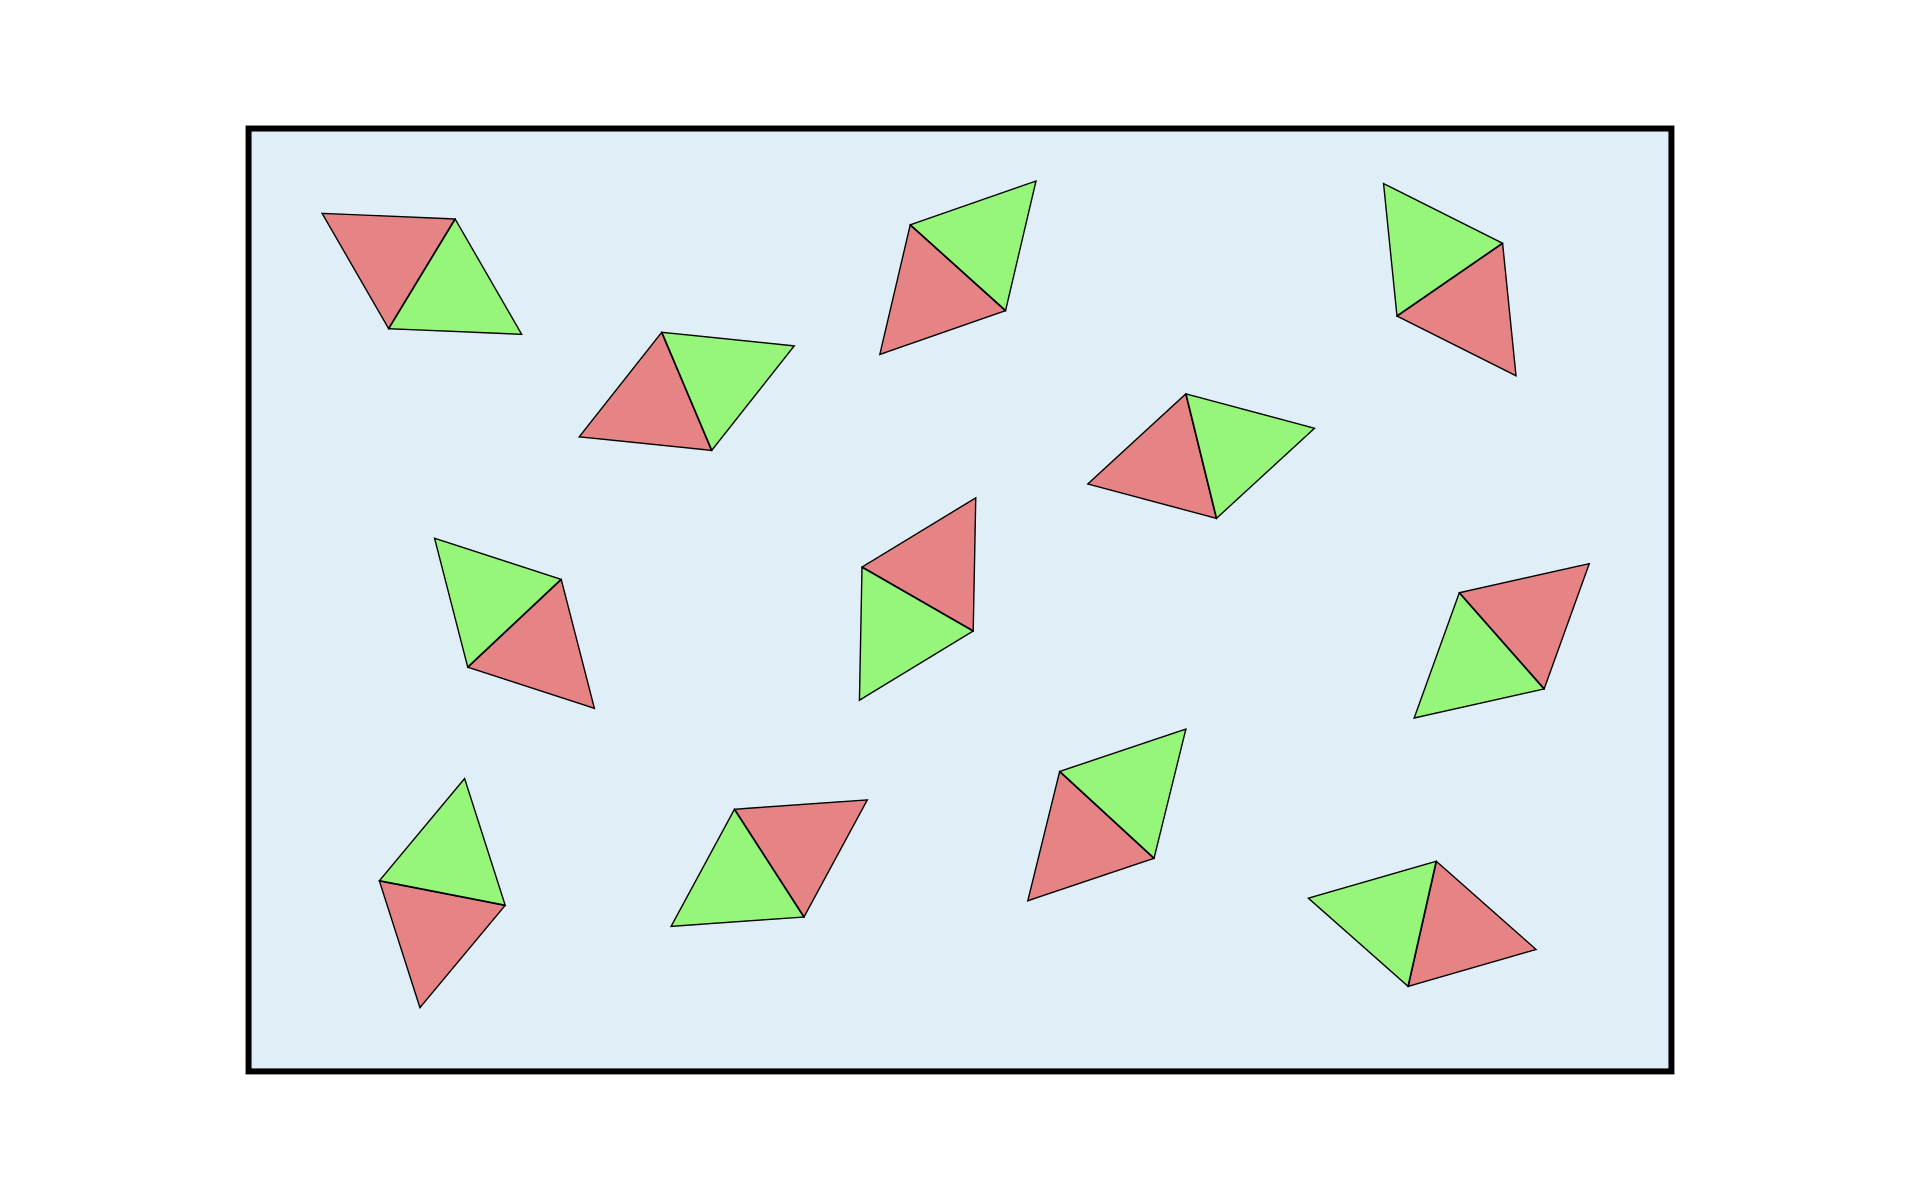
\includegraphics[width=\textwidth]{pics/MS_Paramagnetismus_1.png} %Von Jens Böning (Jensel) - selfmade – selbst gemacht, Gemeinfrei, https://commons.wikimedia.org/w/index.php?curid=506271
		\end{minipage}
		\begin{minipage}{0.32\textwidth}
			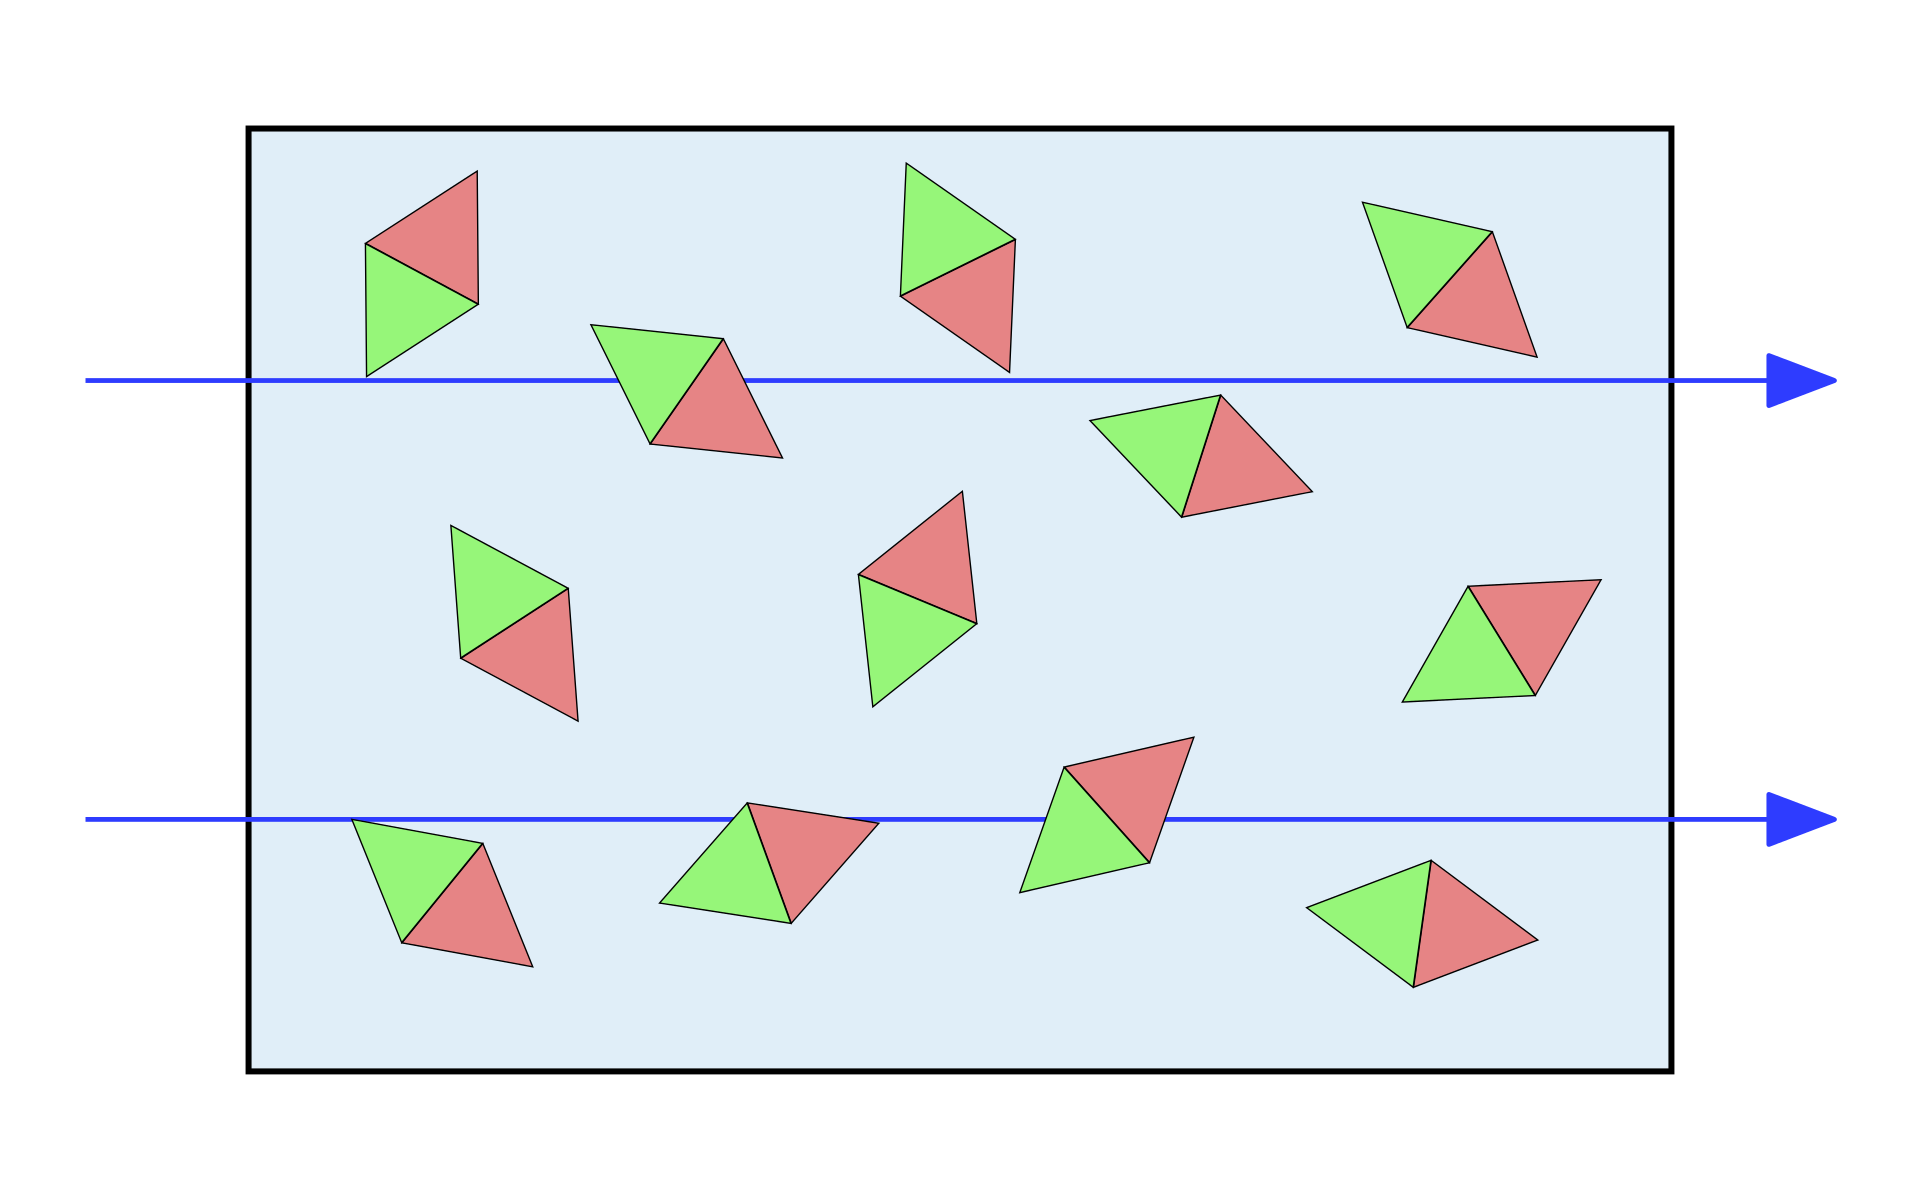
\includegraphics[width=\textwidth]{pics/MS_Paramagnetismus_2.png} %Von Jens Böning (Jensel) - selfmade – selbst gemacht, Gemeinfrei, https://commons.wikimedia.org/w/index.php?curid=506273
		\end{minipage}
		\begin{minipage}{0.32\textwidth}
			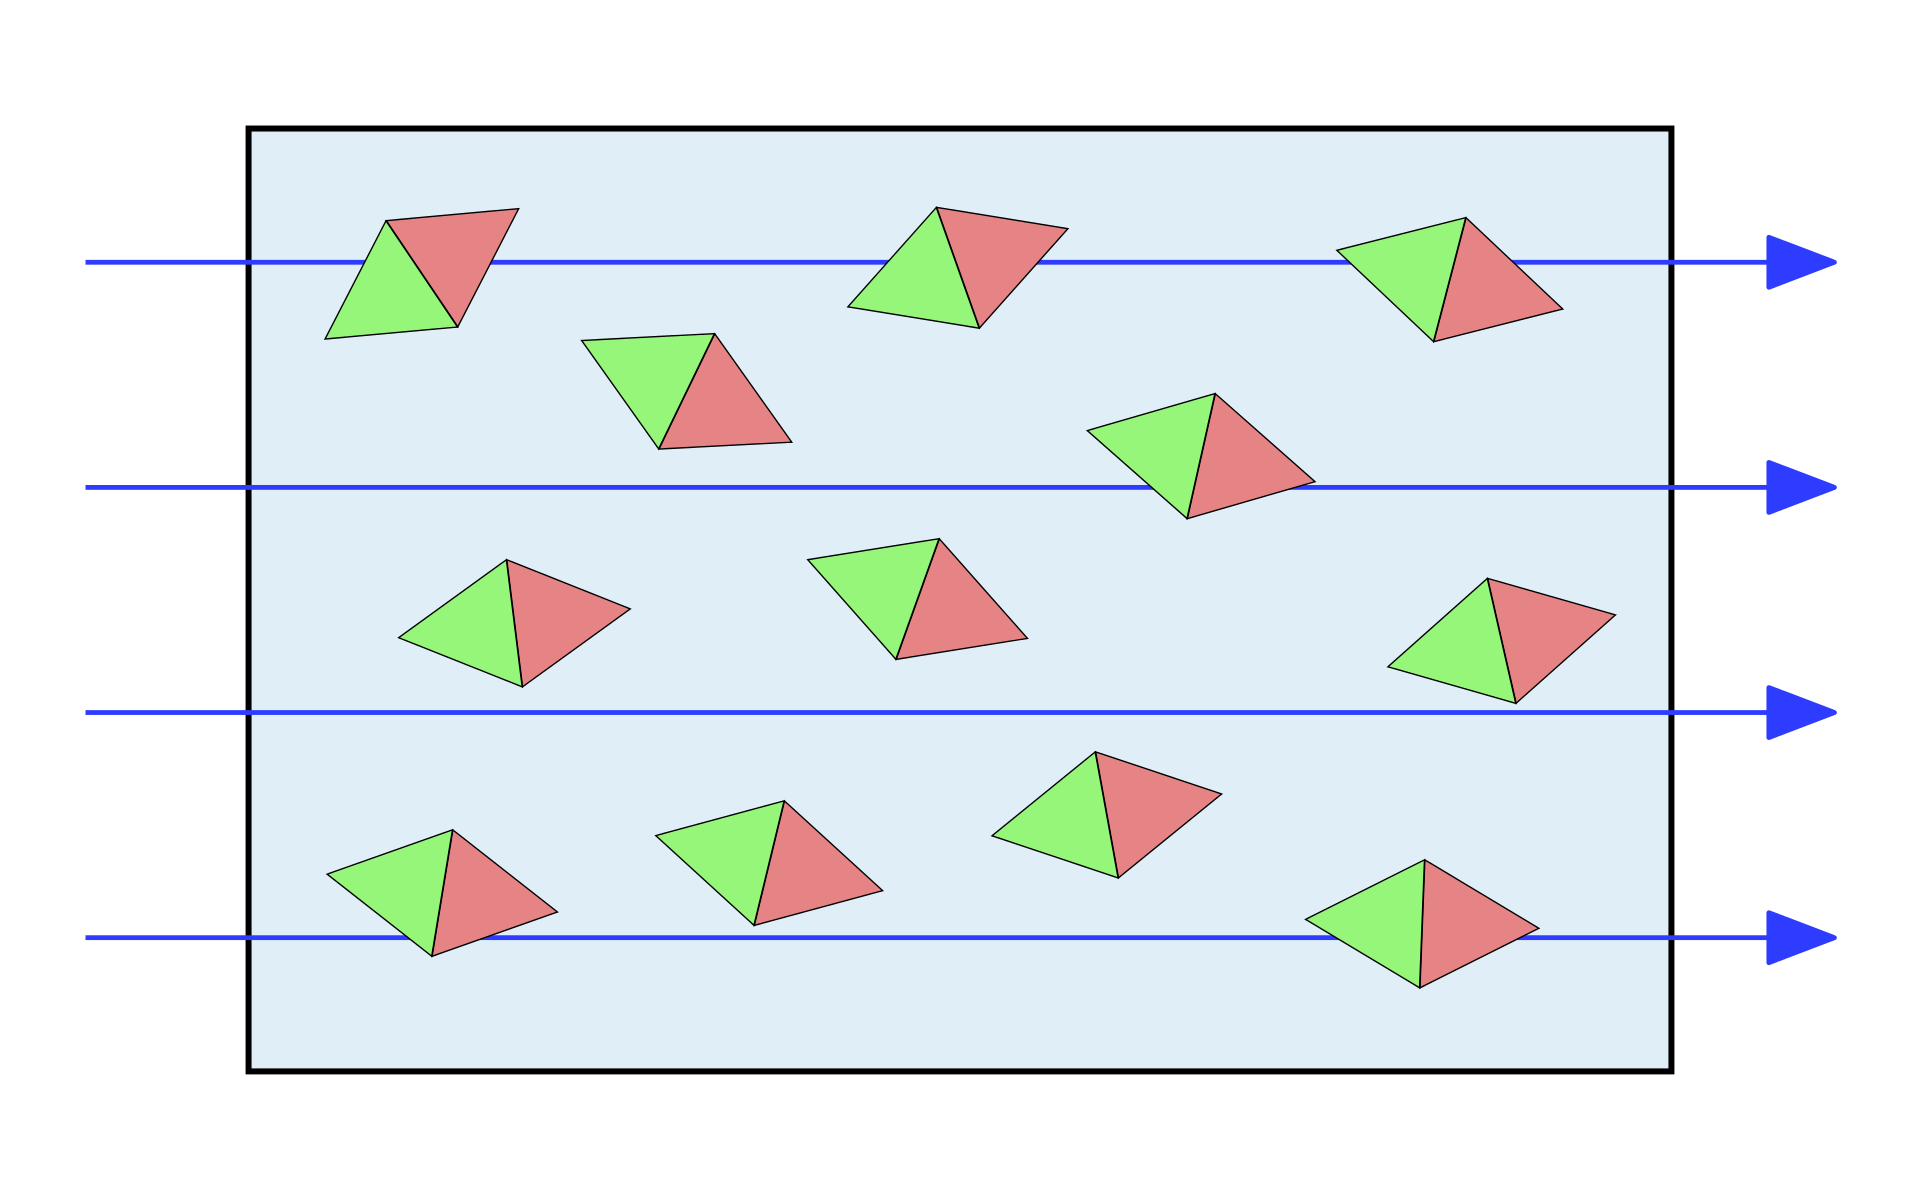
\includegraphics[width=\textwidth]{pics/MS_Paramagnetismus_3.png} %Von Jens Böning (Jensel) - selfmade – selbst gemacht, Gemeinfrei, https://commons.wikimedia.org/w/index.php?curid=506275
		\end{minipage}\\
		\begin{minipage}{0.32\textwidth}
			\center ohne M-feld
		\end{minipage}
		\begin{minipage}{0.32\textwidth}
			\center schwaches M-feld
		\end{minipage}
		\begin{minipage}{0.32\textwidth}
			\center starkes M-feld
		\end{minipage}
	\end{center}
\end{karte}

\begin{karte}{Wie Funktioniert der Ferromagnetismus?}
	\begin{itemize}
		\item Kann magnetisiert werden
		\item Magnetisierung bleibt erhalten
	\end{itemize}
	\center 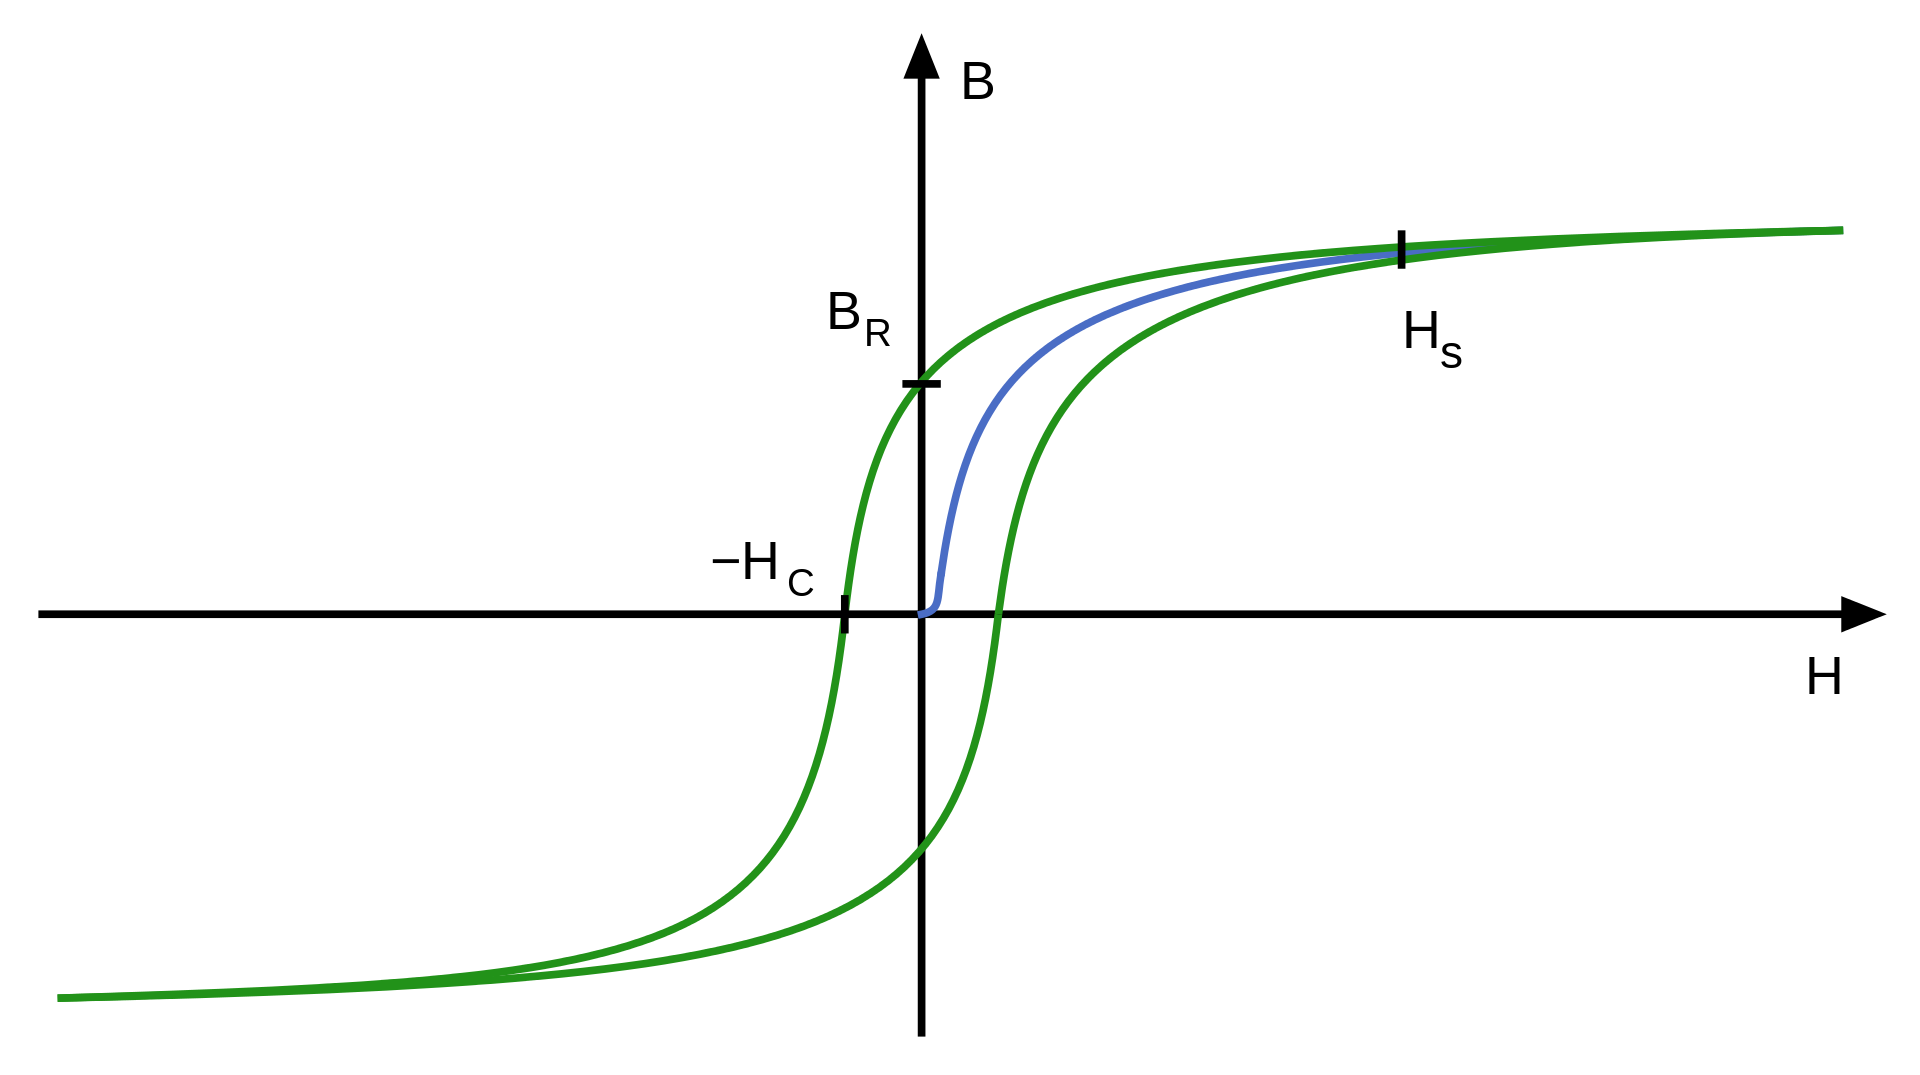
\includegraphics[width=0.6\textwidth]{pics/MS_Ferromagnetismus.png} %Von Walter Dvorak - Eigenes Werk, Gemeinfrei, https://commons.wikimedia.org/w/index.php?curid=10902228
\end{karte}

\begin{karte}{Wie gleichen und unterscheiden sich Ferro- und Ferrimagnetismus?}
	\begin{itemize}
		\item Beide Magnetismen basieren auf Weisschenbezirken
		\item Im Ferromagnetismus sind die Weisschenbezirken parralell ausgerichtet.
		\item Im Ferrimagnetismus sind die Weisschenbezirken mehrheitlich antioarallel ausgerichtet.
		\item Die Ursache sind bei beiden die Spinnmomente.
		\item Ferromagnetische Materialien müssen Leiter sein. Ferrimagnetische Materialien können auch isolatoren sein und sind es üblicherweise auch.
	\end{itemize}
\end{karte}

\begin{karte}{Was bedeuten folgende Begriffe:\\
	\begin{compactitem}
		\item Remanenz
		\item Reluktanz
		\item Hysterese
		\item Permeanz
		\item Koerzitivfeldstärke
	\end{compactitem}}

	\begin{compactitem}
		\item Remanenz: Ist die Restmagnetisierung, wenn das externe Feld entfernt wurde
		\item Reluktanz: Magnetischer Widerstand
		\item Hysterese: Nachwirkung. Es gibt eine Erinnerung. Die Magnetisierung ist nicht direkt reversibel.
		\item Permeanz: Magnetischer Leitwert. Formelzeichen ($\Lambda$), $\dfrac{\mu \cdot A}{l}$
		\item Koerzitivfeldstärke: Ist die Feldstärke welche von aussen auf das Material wirkt um die gesamte Flussdichte $B$ auf $0$ zu bringen um die maximale Remanenz aufzuheben.
	\end{compactitem}
\end{karte}

\begin{karte}{Wie lautet das Ohmischegesetz des Magnetismus?}
	\begin{huge}
		\begin{center}
			$R_{m}=\dfrac{V_{m}}{\Phi}$\\
		\end{center}
	\end{huge}
	Das Analoge zum ohmschen Gesetz $U=R I$ für magnetische Kreise ist $V_{m}=R_{m} \Phi$ (auch als Hopkinsonsches Gesetz bekannt) und folglich muss $R_{m}$ der magnetische Widerstand sein. Er ist in der Fachsprache auch bekannt als Reluktanz.
\end{karte}